\documentclass[11pt,a4paper]{article}
\usepackage[margin=0.62in]{geometry}
\usepackage[T1]{fontenc}
\usepackage{lmodern,microtype,amsmath,amssymb,booktabs,array,graphicx}
\usepackage{algorithm,algpseudocode}
\usepackage[font=small,labelfont=bf]{caption}
\usepackage{enumitem,fancyhdr,xcolor,hyperref}
\hypersetup{colorlinks=true,linkcolor=blue!45!black,urlcolor=blue!45!black,
 pdftitle={Stabilizing Training by Capping Local Representation Displacement},
 pdfauthor={Analysis 065},pdfsubject={Representation-informed local displacement caps}}
\setlength{\parindent}{0pt}
\setlength{\parskip}{5pt}
\setlength{\headheight}{14pt}
\setlist{nosep,leftmargin=1.4em}
\pagestyle{fancy}\fancyhf{}
\fancyhead[L]{\small Local representation displacement caps}
\fancyhead[R]{\small Technical report / Analysis 065}
\fancyfoot[C]{\thepage}
\newcommand{\R}{\mathbb R}
\newcommand{\norm}[1]{\left\lVert#1\right\rVert}
\newcommand{\vecop}{\operatorname{vec}}
\newcommand{\rms}{\operatorname{RMS}}
\newcommand{\sect}[1]{\vspace{2pt}\section*{#1}\vspace{-4pt}}

\begin{document}
\thispagestyle{plain}
{\LARGE\bfseries Stabilizing Training by Capping\\[3pt]
Local Representation Displacement\par}
{\large An intervention motivated by destructive-regime tracing\par}
{\small Analysis 065 / H048 \hfill 8 November 2026}

\sect{Findings at a glance}
We cap the local preactivation change caused by each proposed weight/bias update,
holding current inputs fixed. All layers remain trainable.
Distributed caps reduce mean training loss by \textbf{22.85\%, 16.22\%, and
26.00\%} for MLP/CIFAR-10, ResNet/CIFAR-10, and Transformer/WikiText-2 in the
selected windows; two further MLP initializations improve by 19.43\% and 32.08\%.
Loss excursions shrink despite persistent or more frequent representation reversals.
\textbf{Terminal test loss worsens under the distributed cap in every setup.}
These finite-window optimization results give no generalization or convergence guarantee.

\sect{1. Motivation and diagnostic notation}
We follow the manuscript: update $t$ starts at $\theta_{t-1}$, uses the raw
full-objective gradient $g_t=\nabla\mathcal L(\theta_{t-1})$, and ends at $\theta_t$.
The raw-gradient diagnostics are
\begin{equation}
 \rho_t=\cos(g_t,g_{t-1}),\qquad
 \eta\widehat\kappa_t=1-\rho_t\frac{\norm{g_t}_2}{\norm{g_{t-1}}_2}
 =1-\frac{\langle g_t,g_{t-1}\rangle}{\norm{g_{t-1}}_2^2}.
 \label{eq:gradient-diagnostics}
\end{equation}
Under Adam, the latter measures normalized projected gradient change, not a
Hessian eigenvalue or stability threshold. A zero denominator is undefined.

Let $A_t^\ell$ be a layer's representation after update $t$ on a fixed ordered
probe. Rows retain examples or token/spatial positions; columns retain features.
For $P_\ell$ total scalar entries (rows times columns), define
\begin{equation}
 \delta_t^\ell=\vecop(A_t^\ell-A_{t-1}^\ell),\qquad
 \rho_t^\ell=\frac{\langle\delta_t^\ell,\delta_{t-1}^\ell\rangle}
 {\norm{\delta_t^\ell}_2\norm{\delta_{t-1}^\ell}_2},\qquad
 r_t^\ell=\frac{\norm{\delta_t^\ell}_2}{\sqrt{P_\ell}}.
 \label{eq:trace}
\end{equation}
Thus $r_t^\ell$ is the root mean square change per scalar coordinate, and
$\rho_t^\ell$ concerns representation changes, whereas $\rho_t$ concerns raw
gradients. Negative cosine describes adjacent cancellation (\emph{destructive}
geometry); it does not imply rising loss. Earlier tracing found large reversing
changes at the first MLP projection, throughout ResNet stages, and after attention
despite steadier Transformer embeddings. Temporal SVD revealed concentrated
motion; its window-fitted basis is fixed, although instantaneous directions can
rotate. These observations motivate movement control without proving a unique
initiating layer. We assess loss excursions together with learning progress.
The controller limits amplitude; it uses neither cosine triggers nor SVD vectors.

\sect{2. Adam direction versus parameter increment}
Adam's first and second moments are $m_t$ and $v_t$, respectively:
\begin{equation}
 \begin{aligned}
 m_t&=\beta_1m_{t-1}+(1-\beta_1)g_t,
 &v_t&=\beta_2v_{t-1}+(1-\beta_2)g_t^{\odot2},\\
 \widehat m_t&=m_t/(1-\beta_1^t),
 &\widehat v_t&=v_t/(1-\beta_2^t),\\
 d_t&=\frac{\widehat m_t}{\sqrt{\widehat v_t}+\epsilon},
 &\Delta\theta_t^{\rm Adam}&=-\eta d_t.
 \end{aligned}
 \label{eq:adam}
\end{equation}
Operations are coordinatewise. Moments start at zero only at initialization;
the fork retains their values and global update count. The signed increment
$\Delta\theta_t^{\rm Adam}$ contains the proposed weight and bias changes
$\Delta W_t^{\rm Adam}$ and $\Delta b_t^{\rm Adam}$ for each module.
Without intervention, $\theta_t=\theta_{t-1}-\eta d_t$.
With the cap, $\theta_t=\theta_{t-1}+\Delta\theta_t^{\rm cap}$ instead.
The cap changes the increment, not the current moments or Adam direction.
Implementation scores use the realized increment after storing the native
proposal in FP32; Eq.~\eqref{eq:adam} gives its exact-arithmetic value.

\newpage
\sect{3. Local displacement and the cap}
\textbf{Affine means a weighted sum plus bias.} For one neuron, $z=w^\top h+b$
is its preactivation, before applying an activation such as tanh.
\textbf{Direct affine response} means the change caused by its proposed weight
and bias updates \emph{with the same input $h$}:
$\Delta z_{\rm direct}=(\Delta w)^\top h+\Delta b$.
For $h=2$, $\Delta w=0.1$, $\Delta b=0$, this change is $0.2$.
Earlier-layer updates can also change $h$; that incoming movement
and subsequent nonlinear transformations are outside this direct contribution.

For a module (suppressing $\ell$), $H_{t-1}\in\R^{n\times d}$ contains
probe inputs before update $t$, $W_{t-1}\in\R^{m\times d}$ its weights,
and $b_{t-1}\in\R^m$ its biases. The proposed local preactivation change is
\begin{equation}
 \Delta Z_t^{\rm local}
 =H_{t-1}(\Delta W_t^{\rm Adam})^\top
   +\mathbf1(\Delta b_t^{\rm Adam})^\top\in\R^{n\times m},\qquad
 s_{t,j}=\sqrt{\frac1n\sum_{i=1}^n(\Delta Z_{t,ij}^{\rm local})^2}.
 \label{eq:score}
\end{equation}
Column $j$ contains neuron $j$'s proposed changes across probe rows.
For MLP linear 1, $H_{t-1}$ is $5000\times3072$ and $\Delta Z_t^{\rm local}$
is $5000\times200$. The score is RMS down a column: signs cannot cancel.
It is not a worst-case bound on each example.

For each targeted module $\ell$, pool $s_{t,j}^\ell$ over its units and the
eight untreated updates ending at the fork state $s_0$
(updates $t=s_0-7,\ldots,s_0$). Set $\tau_\ell$ to their
chosen quantile $q$, and keep it fixed. Current inputs and scores are recomputed
each step. For a positive threshold,
\begin{equation}
 a_{t,j}^\ell=\min(1,\tau_\ell/s_{t,j}^\ell),\qquad
 \Delta W_{t,j:}^{\ell,\rm cap}=a_{t,j}^\ell\Delta W_{t,j:}^{\ell,\rm Adam},\qquad
 \Delta b_{t,j}^{\ell,\rm cap}=a_{t,j}^\ell\Delta b_{t,j}^{\ell,\rm Adam}.
 \label{eq:cap}
\end{equation}
Use $a=1$ for a zero score. A zero calibrated threshold disables that module's
cap. The same multiplier scales a neuron's full weight row and bias; all
untargeted increments remain native. Its direct RMS becomes $a_{t,j}s_{t,j}\leq\tau$
in exact arithmetic; storage rounding is checked separately. q50 denotes a calibration median, not a
requirement to modify half the units at each subsequent step.

\begin{algorithm}[H]
\caption{Local representation displacement cap at update $t$}
\label{alg:cap}
\begin{algorithmic}[1]
\Require Parameters $\theta_{t-1}$, Adam state, fixed probe, target modules $\mathcal S$, budgets $\tau_\ell$
\State Capture current module inputs $H_{t-1}^\ell$ on the probe; retain $\theta_{t-1}$.
\State Compute the raw gradient $g_t$ of the complete training objective.
\State Advance $m_t,v_t$ and the clock; form $d_t$ and the stored native proposal $\theta_t^+$.
\State Set $\Delta\theta_t^{\rm Adam}=\theta_t^+-\theta_{t-1}$; initialize $\Delta\theta_t^{\rm cap}=\Delta\theta_t^{\rm Adam}$.
\For{each targeted module $\ell\in\mathcal S$ with $\tau_\ell>0$}
  \State Extract $(\Delta W_t^{\ell,\rm Adam},\Delta b_t^{\ell,\rm Adam})$ from $\Delta\theta_t^{\rm Adam}$.
  \State Compute preactivation changes at fixed inputs and per-unit RMS, Eq.~\eqref{eq:score}.
  \State Scale each proposed weight row and bias using Eq.~\eqref{eq:cap}.
\EndFor
\State Store $\theta_t=\theta_{t-1}+\Delta\theta_t^{\rm cap}$; keep the advanced Adam state.
\State Measure loss and actual consecutive representation changes for evaluation.
\end{algorithmic}
\end{algorithm}

\textbf{Entry versus distributed.} The entry variant targets MLP linear 1,
ResNet conv 1, or the first Transformer QKV projection. The distributed variant
targets both MLP hidden affines, all 31 ResNet convolutions, or both QKV
projections plus all four feed-forward affines. MLP output weights, ResNet
normalization/classifier parameters, and Transformer attention output projections,
LayerNorm, embeddings and decoder are outside the cap. A convolutional score
averages over images and spatial positions; QKV scores measure the projection,
not the complete attention operation. Selection is over existing units/channels,
not temporal singular vectors.

\newpage
\sect{4. Experimental design and measurement timing}
\begin{table}[H]
\centering\small\setlength{\tabcolsep}{4pt}
\begin{tabular}{@{}>{\raggedright\arraybackslash}p{.17\linewidth}>{\raggedright\arraybackslash}p{.27\linewidth}>{\raggedright\arraybackslash}p{.29\linewidth}>{\raggedright\arraybackslash}p{.20\linewidth}@{}}
\toprule
Case & Full objective per update & Fixed probe & LR; fork; final state \\
\midrule
MLP / CIFAR-10 & 5,000 images; half squared output error & All 5,000 images, native 1,000-image chunks & .001; 448; 800/1152 \\
ResNet / CIFAR-10 & 50,000 images; mean cross-entropy & First intact 1,000-image BatchNorm group & .003; 264; 576 \\
Transformer / WikiText-2 & 2,088,600 valid tokens; mean NLL & First 64 length-35 sequences: 2,240 valid positions & .003; 552; 928 \\
\bottomrule
\end{tabular}
\caption{Full-objective deterministic updates throughout. Probe coverage changes only
measurement and the local constraint, not the training objective.}
\end{table}

The MLP is $3072\to200\to200\to10$ with two tanh activations and a linear output.
ResNet-32 has stage widths 16/32/64 and BatchNorm without running statistics.
The two-block Transformer has width 200, two attention heads, feed-forward width
200, zero dropout and untied embeddings/decoder (vocabulary 33,278).
All use Adam $(\beta_1,\beta_2)=(.9,.999)$, $\epsilon=10^{-8}$, no weight decay
or clipping, FP32 parameters and disabled TF32. Dataset order, cached data,
initialization and source/config hashes are pinned. All gradients and moments
continue to update; future gradients naturally depend on the intervened trajectory.
For the MLP, $\mathcal L=(2N)^{-1}\norm{F-Y}_F^2$ with one-hot targets $Y$.
Output diagnostics retain raw linear outputs for MLP and all class/vocabulary
log-probabilities for ResNet/Transformer, without averaging probe rows.


\textbf{Figure indexing.} The horizontal axis retains the recorded number of
completed updates $s$. At $s$, loss is $\mathcal L(\theta_s)$, the next gradient
is $g_{s+1}$, and outgoing motion is $\delta_{s+1}^\ell=\vecop(A_{s+1}^\ell-A_s^\ell)$.
Hence the plotted cosines are $\rho_{s+1}$ and $\rho_{s+1}^\ell$; the gradient
cosine concerns the preceding transition, while the representation cosine includes
the next one. Labels now show this distinction; no recorded state or value is shifted.
The first intervened update is $t=s_0+1$ (e.g., $449$ after MLP state $448$).
\sect{5. Results: cap variants and unchanged-Adam controls}
The primary entry screen uses q75; the common distributed comparison uses q50.
Each branch is paired with unchanged Adam from its exact native fork on the
same worker. Mean loss averages the stated loss states; tail averages the last
32 states; $\mathrm{PV}=\sum_s\max(\mathcal L(\theta_{s+1})-\mathcal L(\theta_s),0)$ uses adjacent states within
that window. Outgoing motion also uses a retained state after its end.
Maximum includes the shared initial state. Percent changes below
are paired descriptive effects; no confidence intervals are claimed.

\begin{table}[H]
\centering\small\setlength{\tabcolsep}{4pt}
\begin{tabular}{@{}llrrrrr@{}}
\toprule
Model & Cap & States & Mean & Tail & Maximum & PV \\
\midrule
MLP & Entry q75 & 448--800 & $-8.26\%$ & $+8.50\%$ & $-37.91\%$ & $-69.50\%$ \\
ResNet & Entry q75 & 264--576 & $-6.29\%$ & $-22.76\%$ & $+21.44\%$ & $-17.15\%$ \\
Transformer & Entry q75 & 552--928 & $-8.53\%$ & $-24.58\%$ & $-14.68\%$ & $-45.20\%$ \\
MLP & Distributed q50 & 448--1152 & $-22.85\%$ & $+4.36\%$ & $-39.04\%$ & $-85.49\%$ \\
ResNet & Distributed q50 & 264--576 & $-16.22\%$ & $-7.48\%$ & $-13.82\%$ & $-46.78\%$ \\
Transformer & Distributed q50 & 552--928 & $-26.00\%$ & $-73.36\%$ & $-79.63\%$ & $-98.81\%$ \\
\bottomrule
\end{tabular}

\caption{Percent changes relative to each branch's own unchanged Adam control.
Negative values mean smaller loss or positive variation. MLP distributed results
use the extended window; the entry screen stops at 800.}
\label{tab:main}
\end{table}

\newpage
\sect{6. Interpretation and sensitivity}


\textbf{Entry caps improve the mean, but not every outcome.} The q75 entry rule
lowers average loss on all three setups, yet increases the MLP tail and ResNet
maximum. It cannot be called a uniform suppression of loss peaks.
\textbf{Distributed q50 improves mean loss and PV in every setup.}
Its MLP tail is 4.36\% worse, while ResNet and Transformer tails improve.
Figure~\ref{fig:entry} shows entry caps; Figure~\ref{fig:distributed} shows
distributed caps, including raw-gradient and actual representation diagnostics.

\begin{table}[H]
\centering\small\setlength{\tabcolsep}{7pt}
\begin{tabular}{@{}llrrr@{}}
\toprule
Model & Additional cap variant & Mean & Tail & PV \\
\midrule
MLP & Entry q50 & $-20.94\%$ & $+13.56\%$ & $-82.03\%$ \\
MLP & Distributed q75 & $-8.44\%$ & $+35.32\%$ & $-71.44\%$ \\
ResNet & Distributed q75 & $-17.42\%$ & $-8.31\%$ & $-17.71\%$ \\
\bottomrule
\end{tabular}

\caption{Scope/quantile checks using the full respective windows (MLP 448--1152;
ResNet 264--576). MLP entry q50 and distributed q50 share a matched worker;
ResNet entry q75 and distributed q75 are also matched.}
\label{tab:sensitivity}
\end{table}

The matched-q50 MLP comparison favors distribution in mean loss
($-22.85\%$ versus $-20.94\%$); the matched-q75 ResNet comparison does too
($-17.42\%$ versus $-6.29\%$). These are joint changes in target scope and the
resulting applied updates, not equal-norm or equal-cost comparisons.
The Transformer entry and distributed experiments also differ in quantile and
GPU architecture (RTX 4090 versus RTX 5090). Their control trajectories differ;
we compare each cap only with its own control and do not claim an isolated
Transformer depth effect. The setup comparisons are not an architecture-only ablation.

\textbf{Stabilization can retain destructive geometry.} Under distributed q50,
the fraction of negative output-change cosines rises from 36.1\% to 66.5\% on
ResNet and from 36.6\% to 97.9\% on Transformer. ResNet's mean output RMS rises
from 0.567 to 0.723 while its maximum falls from 2.785 to 1.592. Transformer
maximum output RMS falls from 15.365 to 1.834. Thus reduced excursions do not
require forward-only motion or smaller movement at every step.

\textbf{Held-out loss limits the claim.} At the terminal state, distributed q50
raises test loss by 2.87\% (MLP seed 0), 8.18\% (ResNet), and 100.17\%
(Transformer). CIFAR-10 evaluation covers all 10,000 test images; WikiText-2
covers all 245,550 supervised test tokens, with token weighting. These are
endpoint comparisons and may reflect different oscillation phases; no held-out
trajectory or generalization improvement is established. MLP replication is
reported on the last page.

\vspace{2pt}{\footnotesize
\textbf{Evidence and reproduction.} Tracing motivation: Analysis 063 technical
report. Cap evidence: H048 Runs 269--274 and 282--283, with exact fork/native
continuation qualification, hash-verified retrieval and retained-state audits.
This report uses only existing verified cap/control records; no new training.
Within Analysis 065, run \path{34_local_cap_report_assets.py}, then
\path{35_build_local_cap_report.py}. Source hashes, table reductions, plotted
values and PDF review are recorded in the accompanying report verification files.
}

\newpage
\begin{figure}[H]
\centering
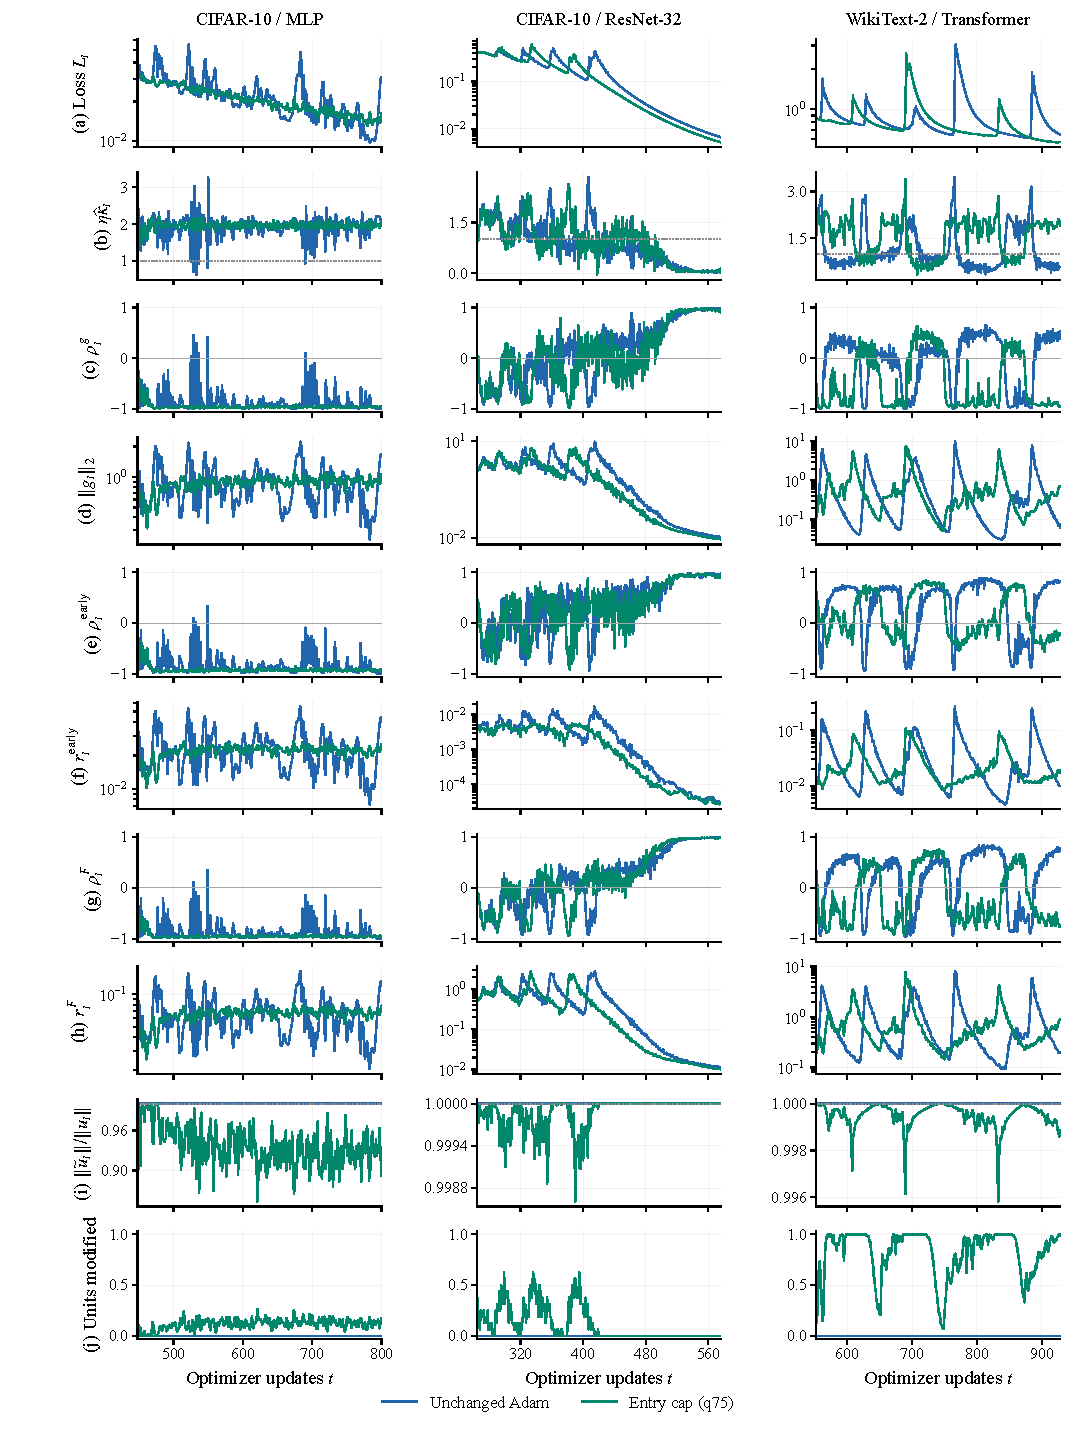
\includegraphics[width=.975\linewidth]{../figures/09-local-cap-entry-manuscript.pdf}
\caption{\textbf{Entry local displacement caps (q75).} Each column compares only
the cap with unchanged Adam on its own worker. Loss, gradient norm and displacement
RMS use logarithmic axes; $\eta\widehat\kappa_{s+1}$ uses a linear axis. Magnitude
scales are independent by column. Early
representation means first MLP tanh, ResNet conv 1 output, or first Transformer
attention output. $\rho$ uses consecutive raw gradients; $\rho^{\rm early}$
and $\rho^F$ use consecutive outgoing representation changes. Row (i) shows the
whole-parameter norm ratio $\gamma_t=\norm{\Delta\theta_t^{\rm cap}}_2/
\norm{\Delta\theta_t^{\rm Adam}}_2$ at $t=s+1$ (undefined for a zero proposal). Row (j)
averages fractions of modified units across targeted modules. All curves are
unsmoothed; zero-denominator cosines are gaps.}
\label{fig:entry}
\end{figure}

\newpage
\begin{figure}[H]
\centering
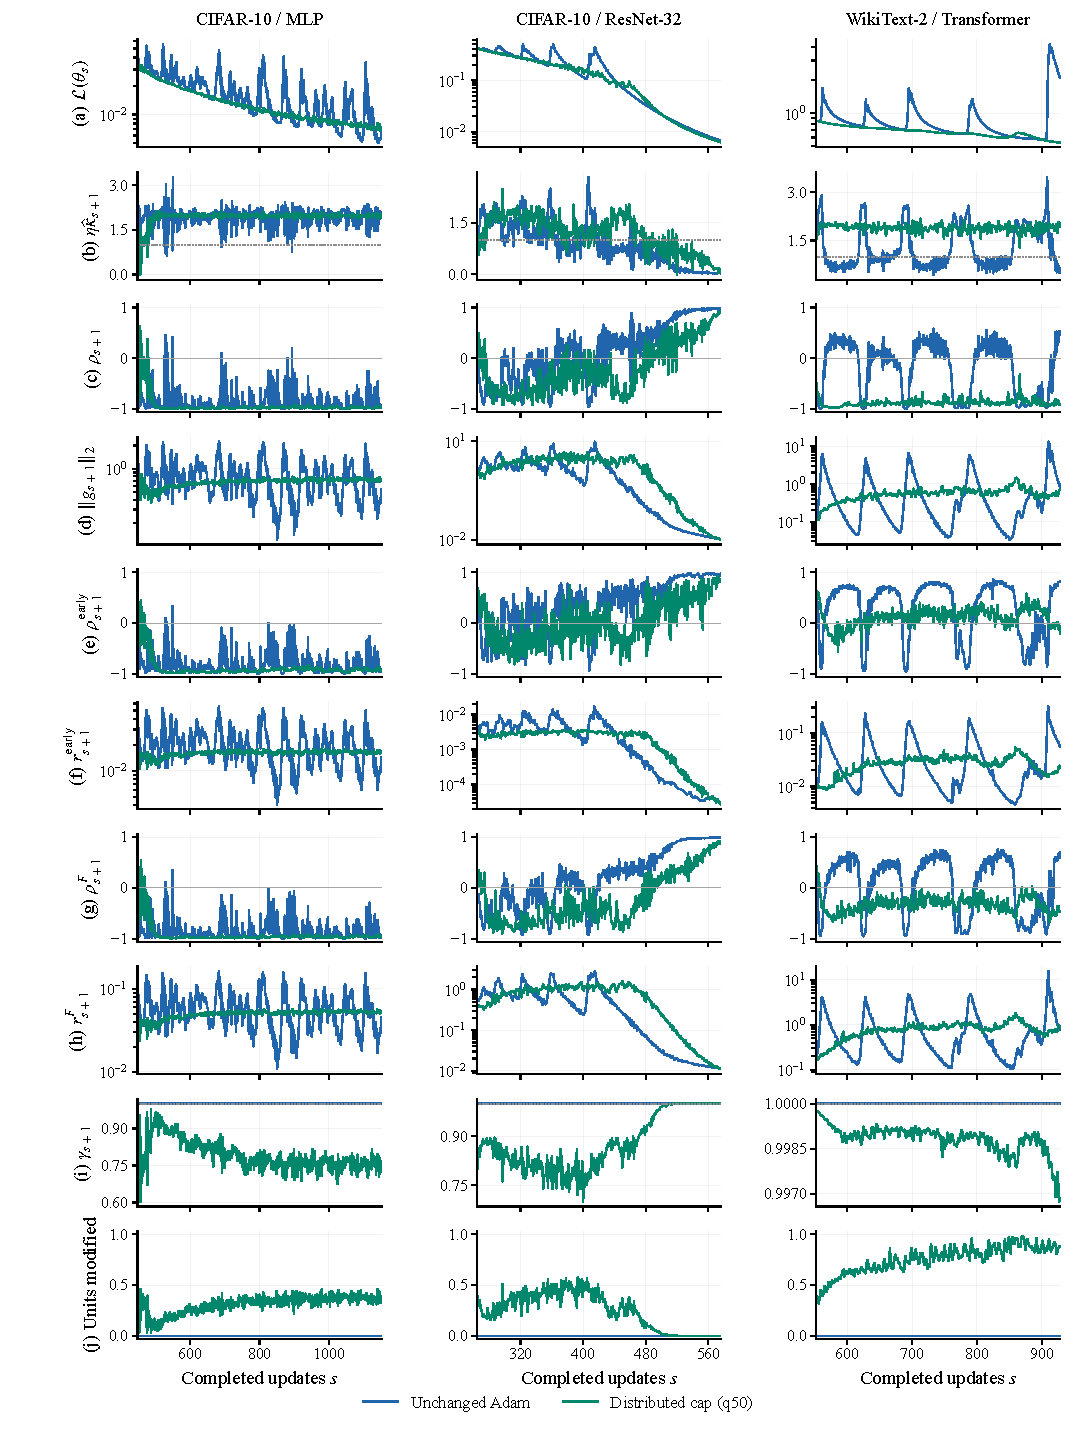
\includegraphics[width=.975\linewidth]{../figures/10-local-cap-distributed-manuscript.pdf}
\caption{\textbf{Distributed local displacement caps (q50).} Same diagnostics
and independent column scales as Figure~\ref{fig:entry}; MLP is extended through
1152. Loss excursions and mean loss decline while output reversals persist.
The Transformer cap targets only 402,000 of 13,828,478 parameters (2.91\%),
so the whole-update norm ratio stays close to one; it is not the fraction of
targeted units modified. This controller bounds direct local contributions,
not complete-network output displacement. Transformer baselines in this figure
and Figure~\ref{fig:entry} come from different GPU architectures and must not
be treated as the same numerical trajectory.}
\label{fig:distributed}
\end{figure}

\newpage
\sect{7. Replication and practical limits}
\begin{figure}[H]
\centering
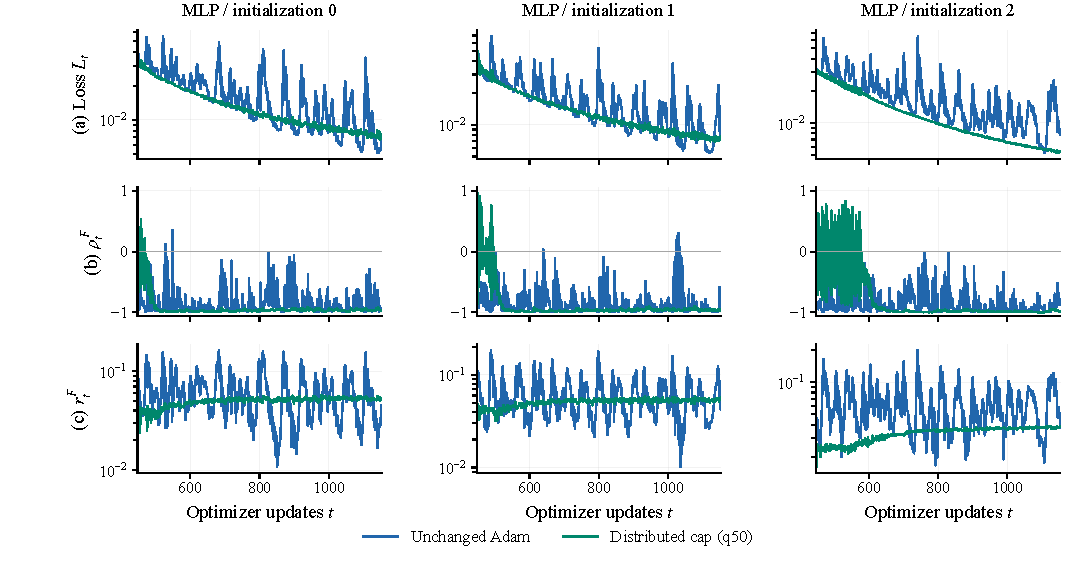
\includegraphics[width=\linewidth]{../figures/11-local-cap-mlp-replication.pdf}
\caption{\textbf{MLP distributed-q50 replication, states 448--1152.}
Initialization 0 selected the candidate; initializations 1/2 received the same
rule without retuning. Loss and output RMS use logarithmic axes with independent
scales per column. Each initialization has its own unchanged Adam control.}
\label{fig:seeds}
\end{figure}
\begin{table}[H]
\centering\small\setlength{\tabcolsep}{9pt}
\begin{tabular}{@{}rrrrr@{}}
\toprule
Initialization & Mean training loss & Tail loss & PV & Terminal test loss \\
\midrule
0 & $-22.85\%$ & $+4.36\%$ & $-85.49\%$ & $+2.87\%$ \\
1 & $-19.43\%$ & $-28.52\%$ & $-73.92\%$ & $+2.76\%$ \\
2 & $-32.08\%$ & $-64.49\%$ & $-82.56\%$ & $+6.13\%$ \\
\bottomrule
\end{tabular}

\caption{Percent changes under distributed q50. Better average training loss
replicates; better terminal test loss does not.}
\end{table}

\textbf{What is bounded.} The preactivation matrix
$Z_t=H_tW_t^\top+\mathbf1b_t^\top$, with incoming change
$\Delta H_t=H_t-H_{t-1}$, has actual change $\Delta Z_t=Z_t-Z_{t-1}$:
\begin{equation}
 \Delta Z_t=\underbrace{H_{t-1}(\Delta W_t^{\rm cap})^\top+\mathbf1(\Delta b_t^{\rm cap})^\top}_{\text{capped direct contribution}}
 +\underbrace{\Delta H_tW_{t-1}^\top+\Delta H_t(\Delta W_t^{\rm cap})^\top}_{\text{incoming movement and interaction}}.
\end{equation}
Only the first term is constrained locally. Nonlinearities, normalization and
attention further transform it. For the first MLP layer, the input is fixed,
so $\Delta H_t=0$. These caps preserve each unit's direct displacement direction
while changing its magnitude; differing factors can change the combined direction.

\textbf{Cost and scope.} The implementation captures probe inputs, evaluates
direct affine products in FP64 and checks final FP32 rounding. It requires no
Jacobian or SVD. Instrumented control/cap seconds per update are 0.01376/0.05797
(MLP), 3.53170/3.83282 (ResNet), and 7.80567/7.95608 (Transformer). Concurrent
Spark work makes the MLP timings non-isolated; these include diagnostics, audit
writes and terminal evaluation, not production optimizer overhead. Fixed prefix
probes and preservation of ResNet's native normalization group are essential;
future padded probes need valid-position masking in local scores too.

\textbf{Conclusion.} Selective representation-amplitude control is a promising
stabilization intervention in these deterministic full-objective continuations.
Three MLP initializations and one per larger model support a limited transfer
result. Selected forks, local calibration, unequal windows and the absence of
stochastic-minibatch tests limit generality. The next validation should compare
additional forks/seeds and repeated held-out measurements at matched training progress.

\end{document}
